\section{Supplementary figures}
\label{sec:appendix-figures}

\skim{UK/Europe model skill.} UK/Europe counterpart of Figure~\ref{fig:model-skill}.

\begin{figure}[htbp]
\centering
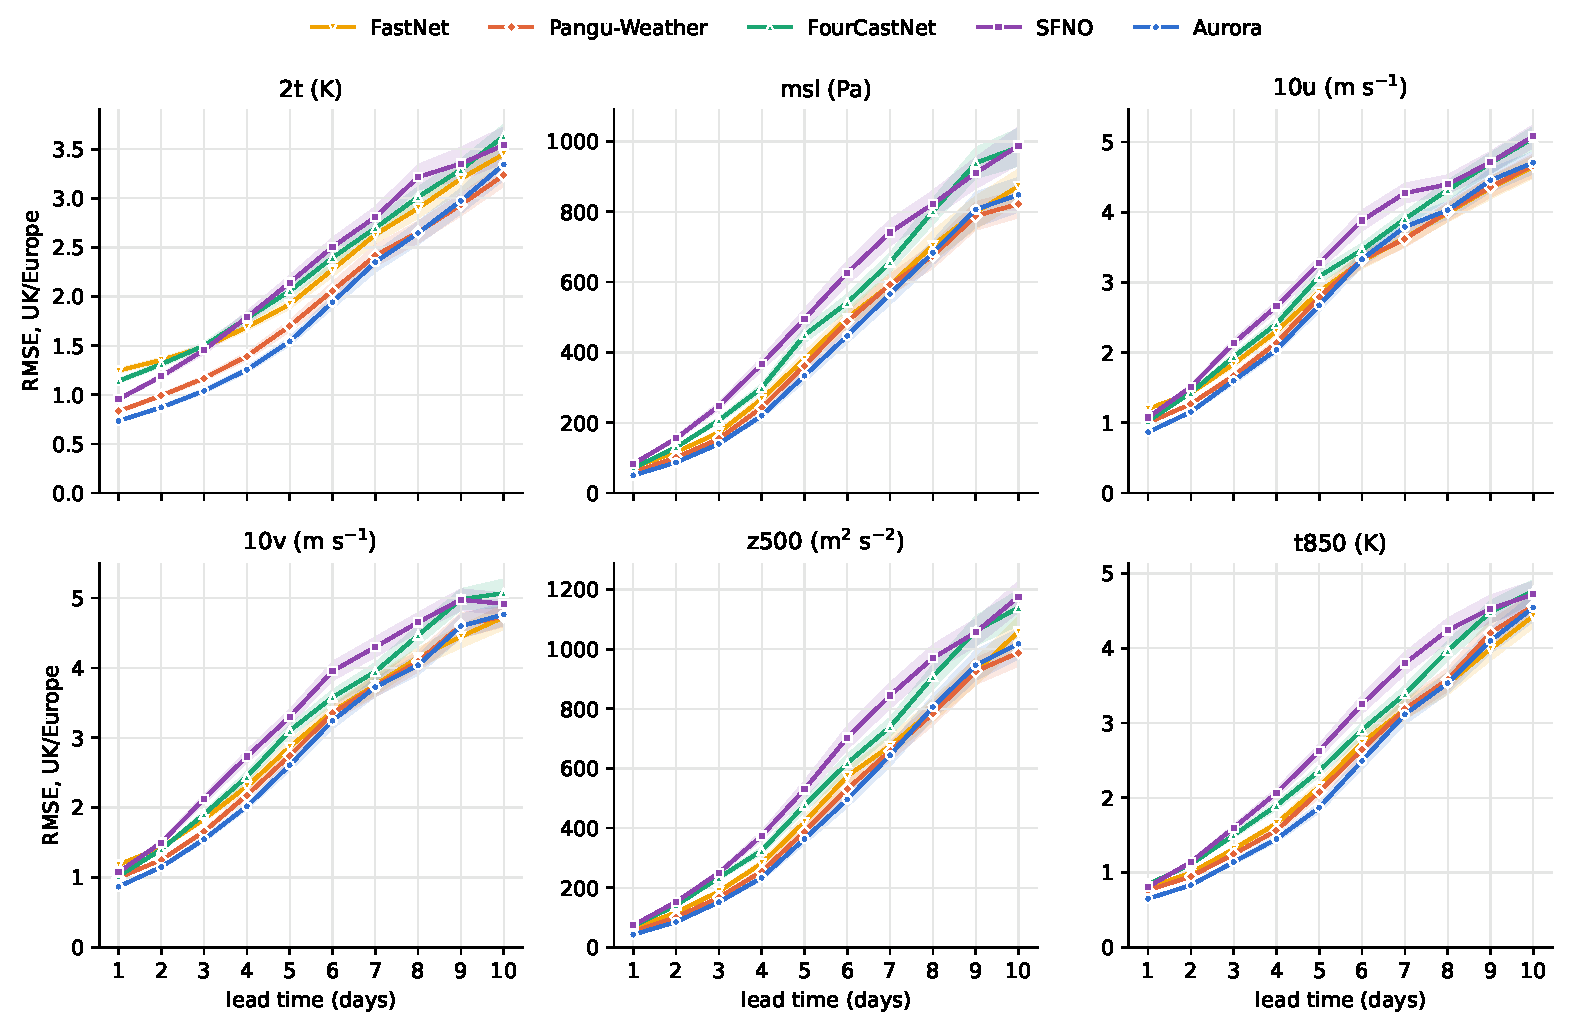
\includegraphics[width=\textwidth]{model_comparison_rmse_uk_europe}
\caption{As Figure~\ref{fig:model-skill}, for the UK/Europe region:
fp32 forecast skill of the models studied, mean RMSE against ERA5 vs.\
lead time.}
\label{fig:model-skill-uk}
\end{figure}

\begin{figure}[htbp]
\centering
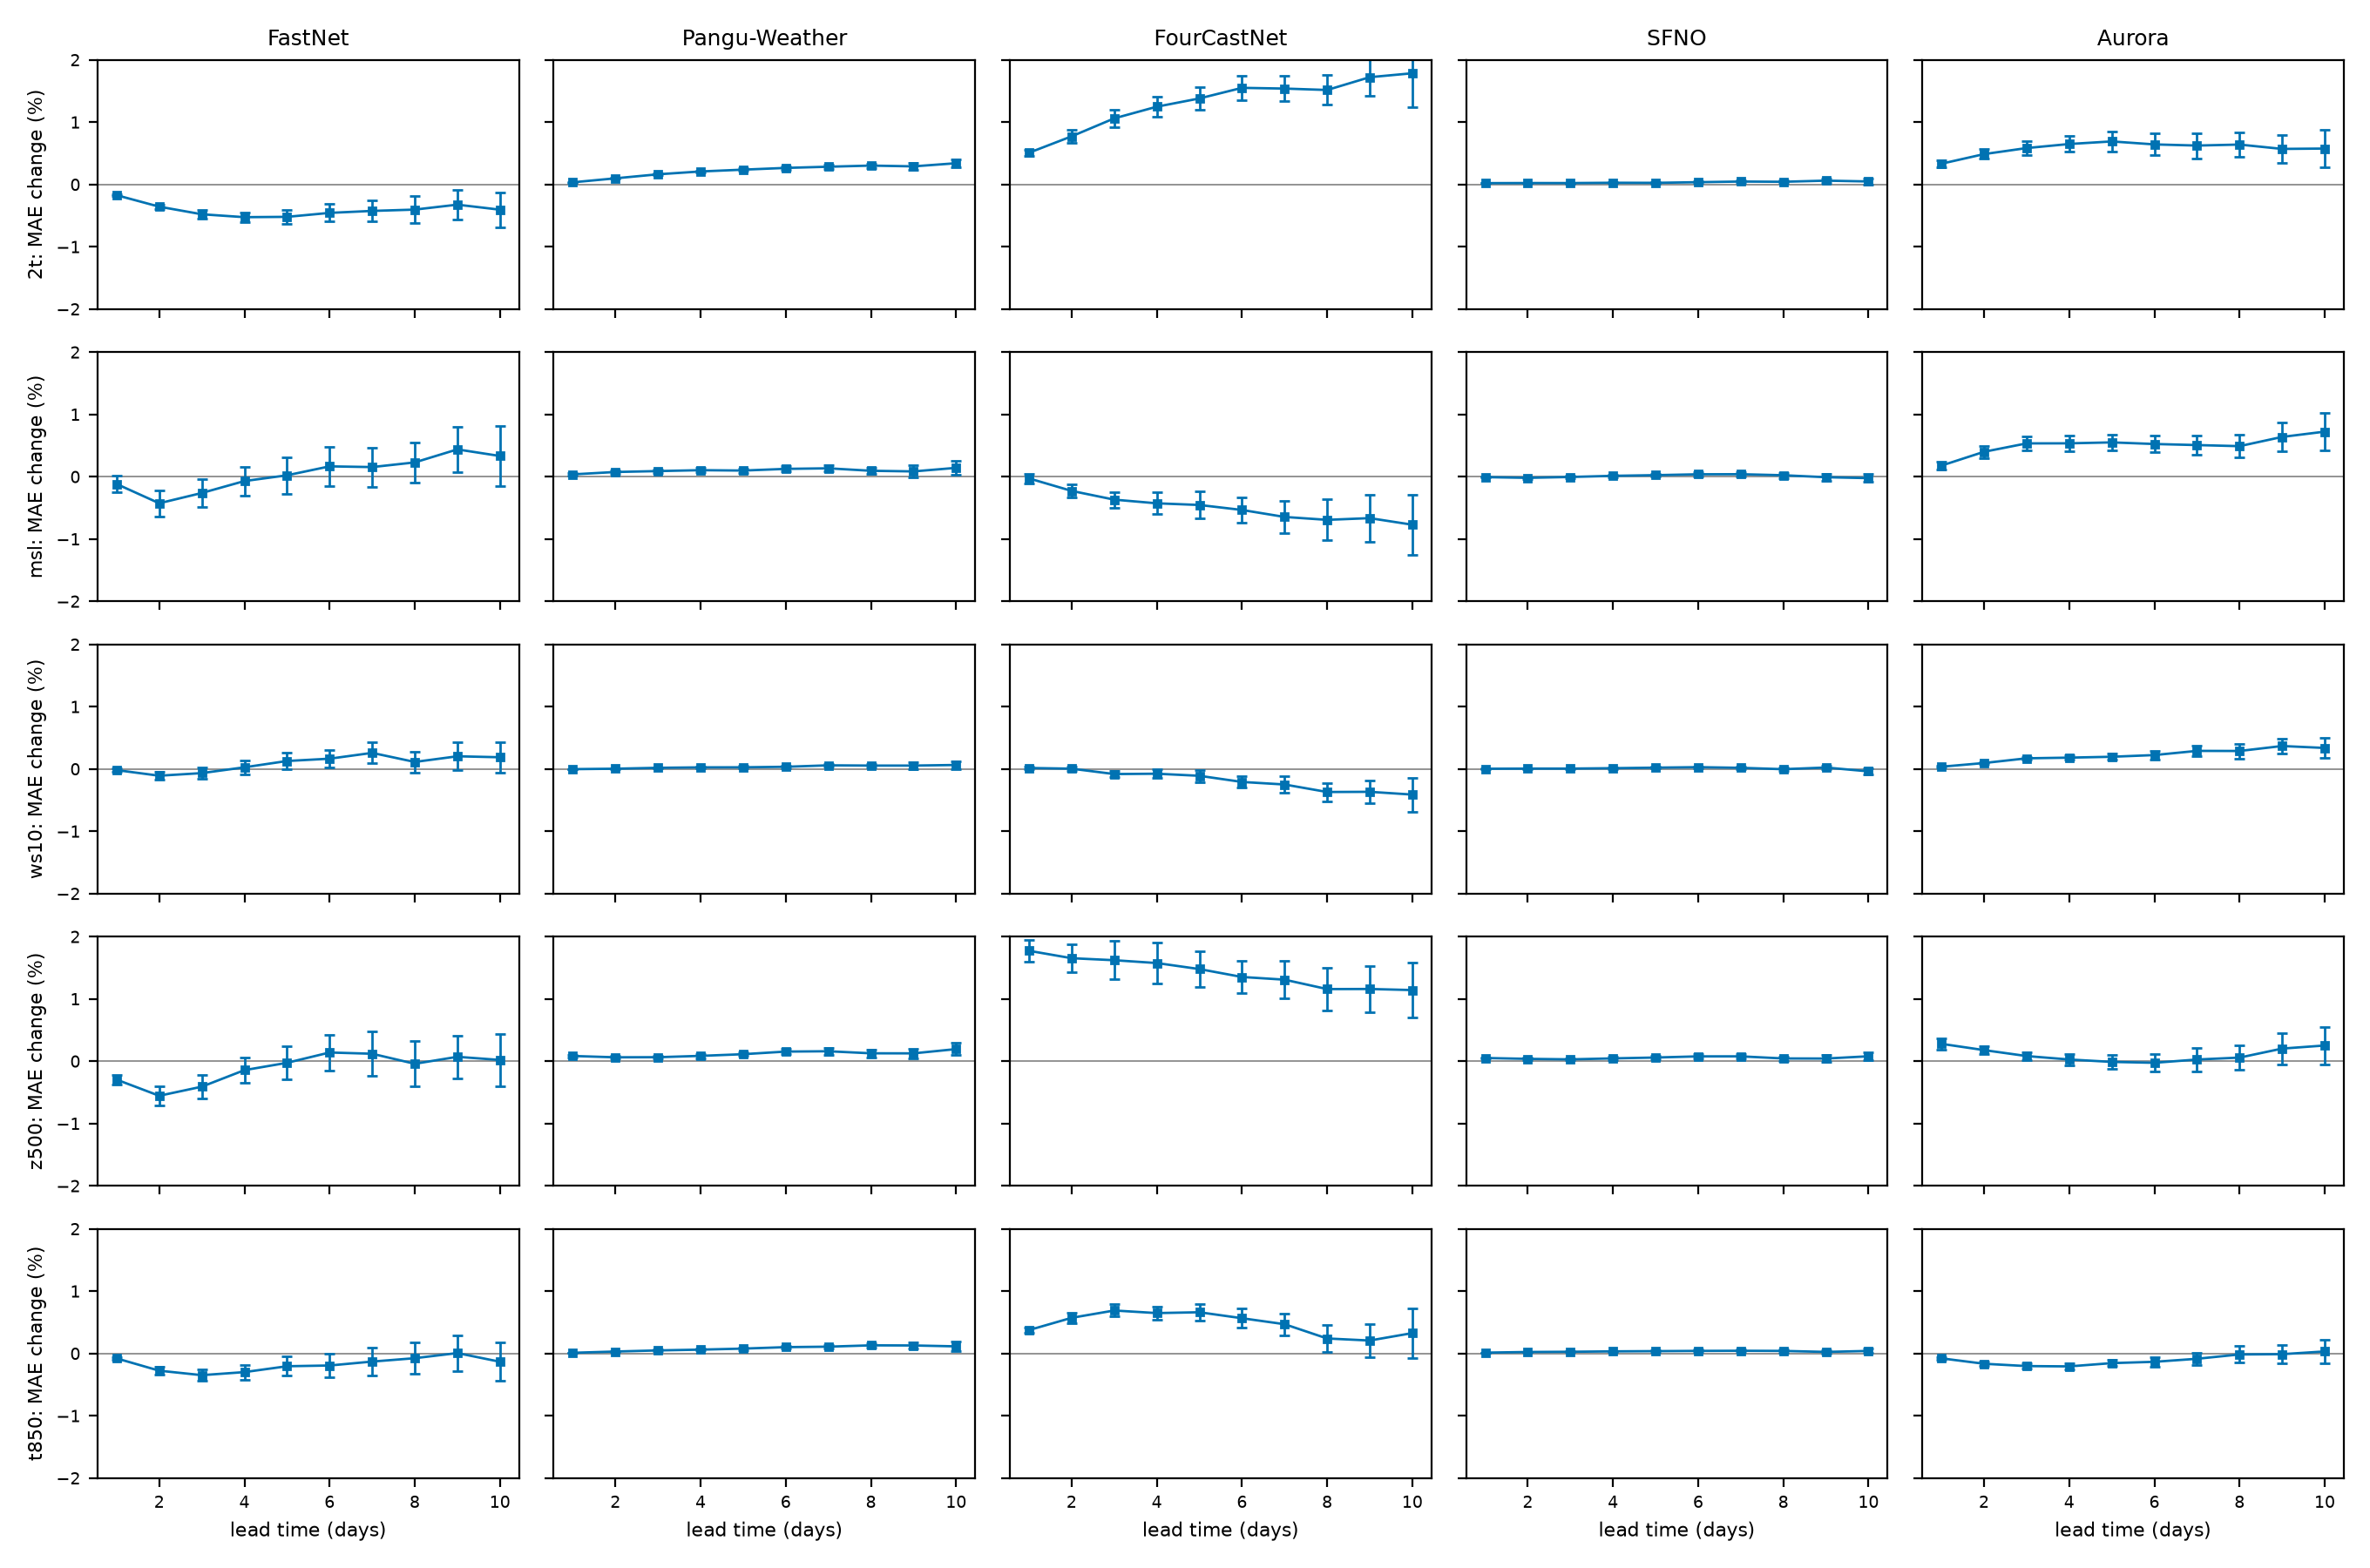
\includegraphics[width=\textwidth]{fp16_vs_fp32_mae_global}
\caption{As Figure~\ref{fig:fp16-rmse}, for the mean absolute error:
change in global MAE against ERA5 of the fp16 forecasts relative to
fp32, with 95\% confidence intervals from the paired per-date
differences; 52 dates in 2024. All panels show $-2$ to $+2\%$;
FourCastNet's intervals for 2t at days 9--10 extend beyond this range.}
\label{fig:fp16-mae}
\end{figure}

\section{Zonal spectra: resolved scales and all wavenumbers}
\label{sec:appendix-spectra}

\skim{Each model's spectra are compared up to the smallest scale it resolves.}
In Figure~\ref{fig:fp16-spectra}, each model's spectra are shown only up
to the smallest scale it resolves. Aurora and Pangu-Weather represent the
atmosphere on patches of $4\times4$ grid points ($1^\circ$), FourCastNet
on patches of $8\times8$ ($2^\circ$), and the detail within a patch is
drawn by a fixed output layer; their fp32 forecasts accordingly show
excess power at the patch wavenumbers (1440/8 = 180 and 1440/4 = 360 and
their multiples). We therefore use wavenumbers just below half the number
of patches around the latitude circle, 179, for Aurora and Pangu-Weather.
For FourCastNet, the limit is lower: its spectral filters act only on
zonal wavenumbers up to 45 (they keep 46 of the 91 zonal Fourier modes of
its $90\times180$ patch grid, which we confirmed by checking that a
filter's contribution to its output has no variance at larger
wavenumbers), so that larger wavenumbers bypass its learned spectral
mixing. For FastNet, the limit is 200, from its grid spacing at the
equator of about $0.9^\circ$; above it, the spectra reflect our
interpolation to $0.25^\circ$. FastNet's interpolated fields also have a
gap at the $0^\circ$ meridian and empty rows at the poles; the gap is
filled by periodic linear interpolation along the latitude circle, and
the empty rows are left out. For SFNO, the limit is 239: the model
truncates its input to spherical harmonics with zonal wavenumbers below
240 and works on an internal grid of 480 longitudes. ERA5 itself has no
variance above wavenumber 639, the truncation of the model from which its
$0.25^\circ$ fields are derived.

\begin{figure}[htbp]
\centering
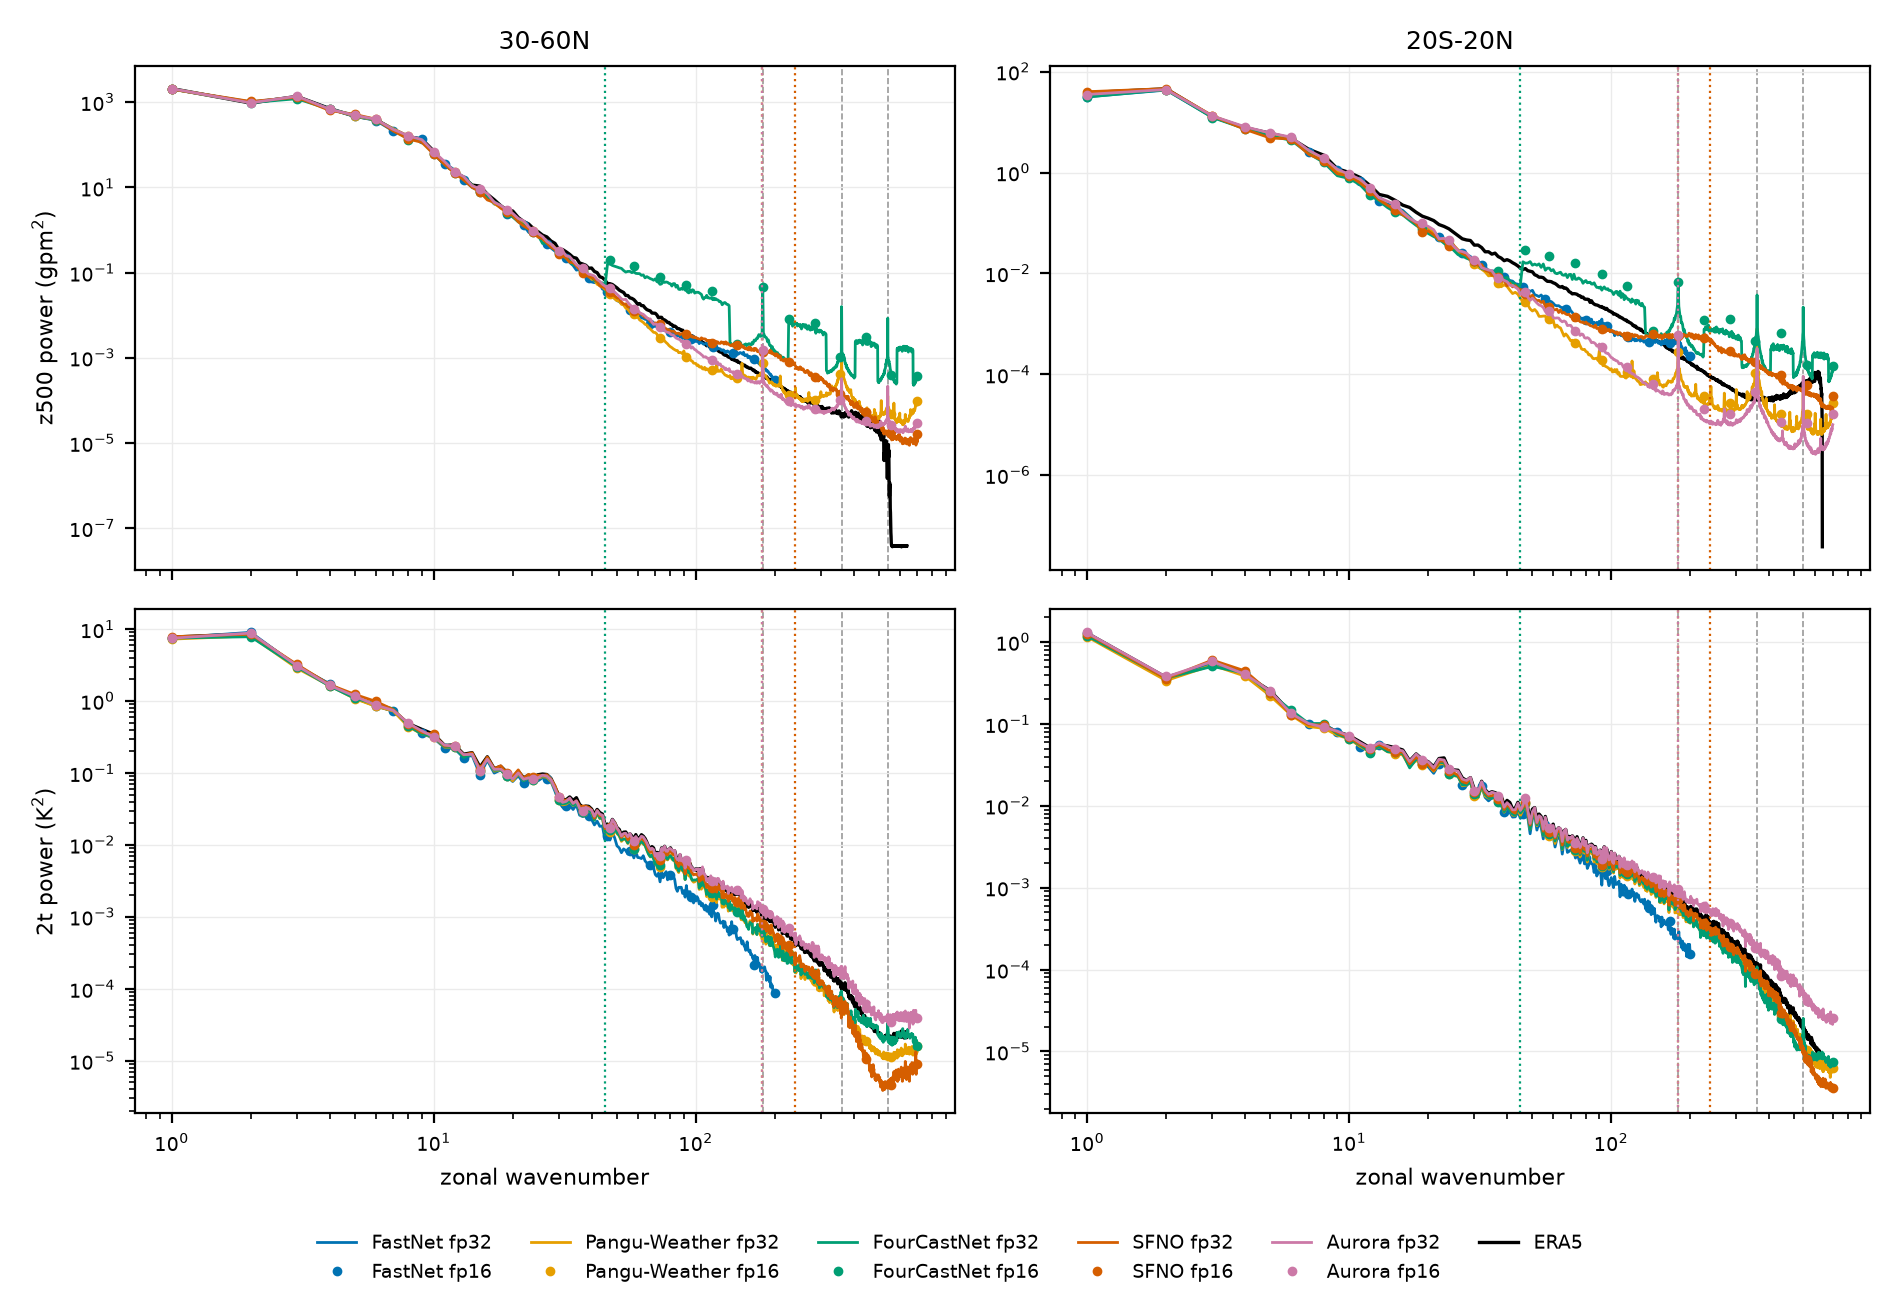
\includegraphics[width=\textwidth]{fp16_spectra_full}
\caption{As Figure~\ref{fig:fp16-spectra}, at wavenumbers up to 700 (ERA5
up to 639, FastNet up to its limit of 200). Dotted: the limit used in
Figure~\ref{fig:fp16-spectra} for each model (colour); dashed grey: the
wavenumbers of FourCastNet's patches (180) and their multiples, at which
also Aurora's and Pangu-Weather's patches (360) leave an imprint.}
\label{fig:fp16-spectra-full}
\end{figure}

\skim{Above the resolved scales, the spectra show the imprint of the models' architectures; fp16 does not change it.}
Figure~\ref{fig:fp16-spectra-full} shows the spectra beyond the
scales the models resolve. The patch architectures leave sharp peaks at
the patch wavenumbers: at 180, 360 and 540 for FourCastNet ($8\times8$
patches) and Aurora, and at 360 for Pangu-Weather ($4\times4$ patches).
FourCastNet's z500 spectrum jumps by an order of magnitude at wavenumber
46, the first wavenumber its spectral filters do not act on, and stays
10--100 times above ERA5's, with further steps towards smaller scales.
These features are much weaker or absent in 2t, which has more variance
of its own at these scales. FastNet, whose forecasts we interpolate from
its $0.9^\circ$ grid, shows none of them. The ERA5 spectrum ends at
wavenumber 639, the truncation of the model from which its $0.25^\circ$
fields are derived. The fp16 spectra lie on the fp32 spectra throughout,
except for FourCastNet's z500 above wavenumber 45, where fp16 adds
variance: rounding noise there is not damped by the model's spectral
filters.

\section{bf16 compared with fp16}
\label{sec:appendix-bf16}

\skim{Converted as a whole, Aurora loses much of its skill in bf16.}
Figure~\ref{fig:rmse-grid-naive} shows the RMSE of Aurora's bf16 forecasts
when the whole model is converted, so that it also holds its state in bf16
in physical units (\S\ref{sec:results-state}), compared with the bf16
network with the state in fp32. The whole-model conversion raises the
RMSE by 19--167\%, the bf16 network alone by at most 25\%.

\begin{figure}[tbp]
\centering
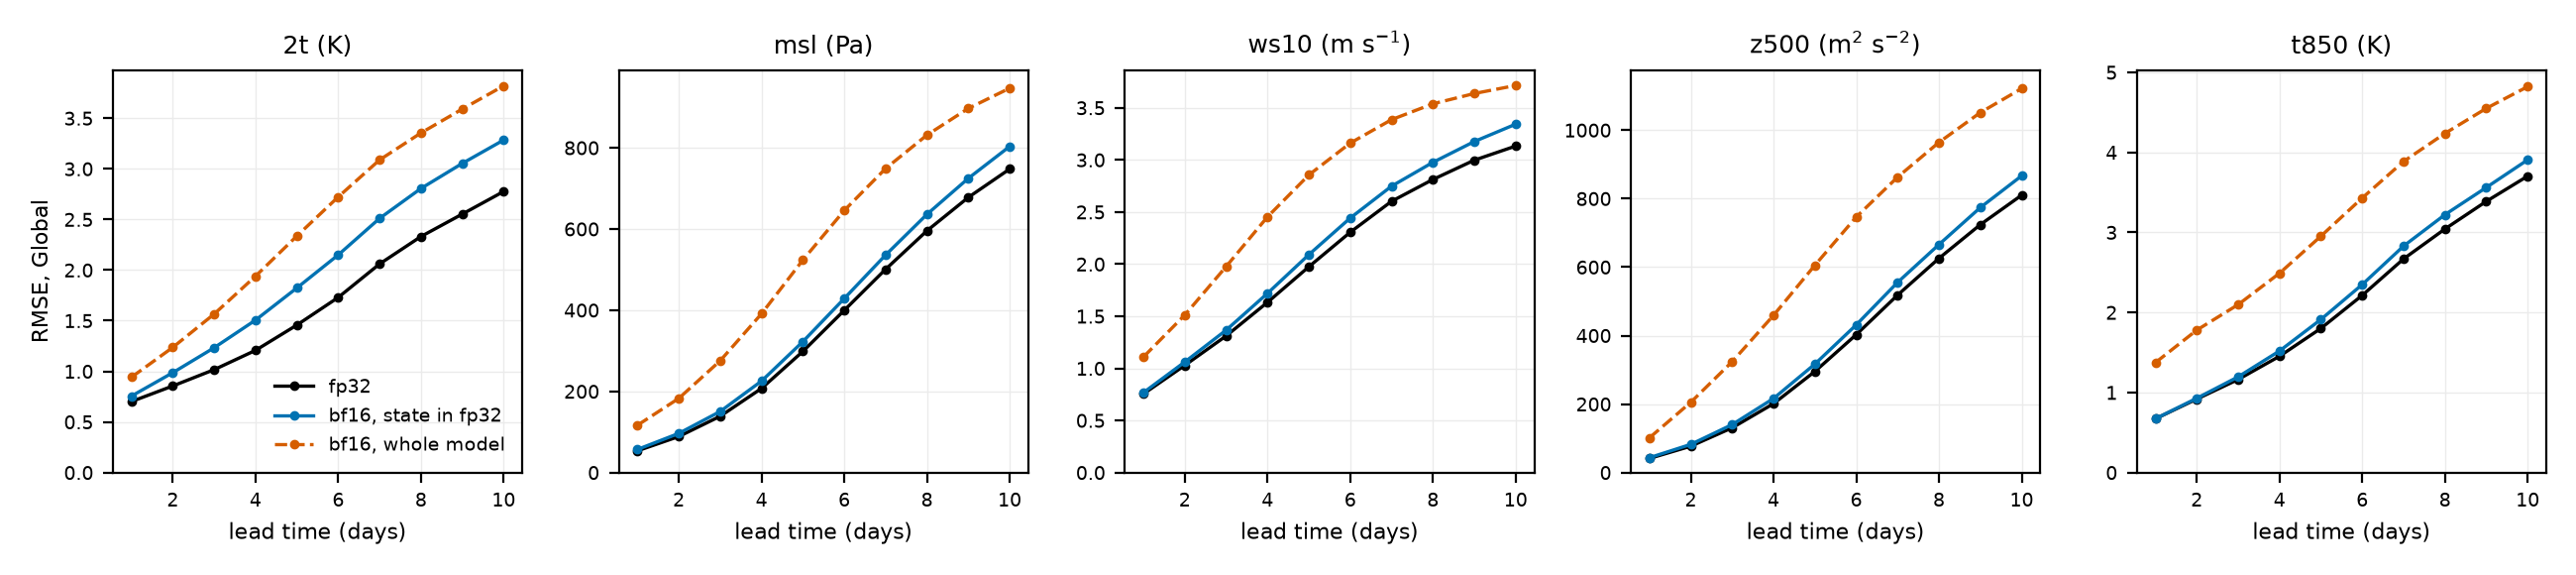
\includegraphics[width=\textwidth]{aurora_bf16_whole_global}
\caption{Mean global RMSE against ERA5 of Aurora's fp32 forecasts, of its
forecasts with the network in bf16 and the state in fp32, and of its
forecasts with the whole model converted with
\texttt{model.to(torch.bfloat16)}, which also rounds the state in physical
units; 52 dates in 2024.}
\label{fig:rmse-grid-naive}
\end{figure}

\begin{table}[htbp]
\centering
\scriptsize
\setlength{\tabcolsep}{3pt}
\caption{Change in global RMSE (\%) relative to fp32 with the network in bf16 and in fp16 (state in fp32 in both), 52 dates in 2024. Bold: significant at the 5\% level (paired $t$-test).}
\label{tab:bf16}
\begin{tabular}{llrrrrrrrrrrrr}
\toprule
 & & \multicolumn{4}{c}{z500} & \multicolumn{4}{c}{2t} & \multicolumn{4}{c}{msl} \\
Model & Precision & d1 & d3 & d5 & d10 & d1 & d3 & d5 & d10 & d1 & d3 & d5 & d10 \\
\midrule
FastNet & bf16 & \textbf{+1.1} & \textbf{+2.1} & \textbf{+3.0} & -0.6 & \textbf{+0.2} & \textbf{+0.6} & \textbf{+0.8} & -0.2 & \textbf{+1.0} & \textbf{+1.7} & \textbf{+1.9} & \textbf{-2.0} \\
 & fp16 & \textbf{-0.3} & \textbf{-0.3} & +0.1 & 0.0 & \textbf{-0.1} & \textbf{-0.2} & \textbf{-0.2} & -0.1 & \textbf{-0.1} & \textbf{-0.2} & +0.1 & +0.3 \\
\midrule
Pangu-Weather & bf16 & \textbf{+3.1} & \textbf{+1.0} & \textbf{+0.6} & +0.7 & \textbf{+0.7} & \textbf{+0.3} & 0.0 & -0.6 & \textbf{+0.6} & \textbf{+0.5} & +0.4 & +0.4 \\
 & fp16 & \textbf{+0.1} & \textbf{+0.1} & \textbf{+0.1} & \textbf{+0.2} & \textbf{0.0} & \textbf{+0.1} & \textbf{+0.1} & \textbf{+0.2} & \textbf{0.0} & \textbf{+0.1} & \textbf{+0.1} & \textbf{+0.2} \\
\midrule
FourCastNet & bf16 & \textbf{+66.4} & \textbf{+28.9} & \textbf{+16.8} & \textbf{+28.5} & \textbf{+14.6} & \textbf{+19.4} & \textbf{+20.0} & \textbf{+271.4} & \textbf{+11.0} & \textbf{+10.2} & \textbf{+8.5} & \textbf{+23.0} \\
 & fp16 & \textbf{+1.4} & \textbf{+0.6} & \textbf{+0.2} & -0.2 & \textbf{+0.2} & \textbf{+0.4} & \textbf{+0.5} & -0.6 & 0.0 & \textbf{-0.2} & \textbf{-0.3} & \textbf{-0.7} \\
\midrule
SFNO & bf16 & \textbf{+0.9} & 0.0 & 0.0 & +0.1 & \textbf{+0.8} & \textbf{+1.0} & \textbf{+1.0} & +0.4 & \textbf{+2.0} & \textbf{+1.0} & \textbf{+0.4} & -0.1 \\
 & fp16 & \textbf{0.0} & \textbf{0.0} & \textbf{+0.1} & 0.0 & \textbf{0.0} & \textbf{0.0} & \textbf{0.0} & 0.0 & \textbf{0.0} & 0.0 & \textbf{0.0} & 0.0 \\
\midrule
Aurora & bf16 & \textbf{+5.4} & \textbf{+7.2} & \textbf{+7.3} & \textbf{+7.0} & \textbf{+7.7} & \textbf{+21.3} & \textbf{+25.2} & \textbf{+18.3} & \textbf{+6.3} & \textbf{+8.5} & \textbf{+8.1} & \textbf{+7.4} \\
 & fp16 & \textbf{+0.2} & \textbf{+0.1} & \textbf{+0.1} & \textbf{+0.3} & \textbf{+0.1} & \textbf{+0.1} & \textbf{+0.2} & +0.1 & \textbf{+0.1} & \textbf{+0.3} & \textbf{+0.2} & \textbf{+0.5} \\
\bottomrule
\end{tabular}
\end{table}


\skim{bf16 costs more skill than fp16 for every model, by up to two orders of magnitude.}
Table~\ref{tab:bf16} compares the change in global RMSE with the
network in bf16 and in fp16, the state in fp32 in both, on the 52 dates.
For every model, the bf16 penalty exceeds the fp16 change at almost
every lead time, by one to two orders of magnitude for Aurora and
FourCastNet. FourCastNet's bf16 forecasts degrade widely by day 10: its
2t error is more than twice that of fp32 on 21 of the 52 dates. Where
bf16 does better than fp32, the differences are small and, except for
FastNet's msl at day 10 ($-2.0\%$), not significant.

\section{Numerical details of the reduced-precision runs}
\label{sec:appendix-precision}

\skim{16-bit arithmetic on the GPU: products in 16 bits, sums in fp32, results rounded.}
On current NVIDIA GPUs, fp16 and bf16 matrix multiplications and
convolutions run on tensor cores, which multiply 16-bit inputs but
accumulate the products in fp32 within each operation, rounding only the
output to 16 bits. PyTorch's 16-bit normalisation, softmax and reduction
kernels likewise typically accumulate internally in fp32. The dominant
error of a 16-bit network is therefore the rounding of every stored
tensor -- the weights once, the intermediate results after every
operation -- which compounds with network depth and, in an
autoregressive forecast, from step to step. One PyTorch default
qualifies this: 16-bit matrix multiplications may use reduced-precision
reductions in some algorithms
(\texttt{allow\_fp16\_reduced\_precision\_reduction} and
\texttt{allow\_bf16\_reduced\_precision\_reduction}, both enabled by
default).

\skim{The fp32 runs use TF32 for convolutions, PyTorch's default, kept deliberately.}
PyTorch allows convolutions to use TF32, a format with fp32's 8-bit
exponent and a 10-bit mantissa (\texttt{cudnn.allow\_tf32}, enabled by
default), whereas fp32 matrix multiplications do not use it by default.
We verified on the GPU used here that this setting is active: an fp32
convolution's relative error against an fp64 reference is
$3\times10^{-4}$ with it, $4\times10^{-7}$ without it, and
$3\times10^{-3}$ in bf16. In this study, ``fp32'' therefore means fp32
for every matrix multiplication and TF32 for the convolutions, which
occur in the patch embeddings of Aurora, Pangu-Weather and FourCastNet
and in Pangu-Weather's patch recovery, and in SFNO's encoder, decoder and
the $1\times1$ convolutions of its blocks -- in the fp32 references and
in the fp32 components of the one-at-a-time runs alike. FastNet contains
no convolutions. We kept this default deliberately, so that the
reference is the model as a typical user runs it, not a strictly fp32
configuration that requires changing library settings.

\skim{FourCastNet needs one change to its code to run in 16 bits.}
FourCastNet's spectral filter layer converts its intermediate results to
fp32 before each Fourier transform, which therefore runs in fp32, and
then multiplies them with the weights, which fails once the weights are
in 16 bits. We convert the results back to the precision of the weights
after the transform. With fp32 weights, the modified model gives
bit-identical results to the original.

\skim{SFNO's complex filters are applied as real and imaginary parts in 16 bits.}
SFNO's spectral filters are complex-valued. PyTorch (version~2.14, used
for every model in this study) has no complex counterpart of bf16, and
its complex fp16 type lacks the batched matrix products the filters need
on the GPU. In bf16 and fp16, we therefore store the real and imaginary
parts of each filter as separate weights in that precision and carry out
the complex multiplication with four real products. PyTorch's standard
conversion of a whole model to 16 bits cannot be used for SFNO: it keeps
only the real parts of complex weights. SFNO's spherical harmonic
transforms always run in fp32, as NVIDIA's implementation prescribes.

\skim{Integer and fp8 quantisation of Aurora: slower than bf16, little memory saved, or out of memory.}
We tested integer and 8-bit floating-point quantisation on Aurora at
full resolution with the \texttt{torchao} library. Weight-only int8 and
fp8 quantisation was 27--28\% \emph{slower} per step than bf16, because
the weights are converted back before every multiplication in a forward
pass whose speed is limited by computation rather than memory access,
and reduced peak memory by only about 10\%, since the intermediate
results, not the weights, dominate memory use. Quantising both weights
and intermediate results to int8 or fp8 ran out of memory on the 16\,GB
GPU, and benchmarks of isolated matrix multiplications showed dynamic
int8 two to seven times slower than bf16, with mixed results for fp8.
Some operations also run in fp32 even in the 16-bit networks;
FourCastNet's Fourier transforms and SFNO's spherical harmonic
transforms, for example.
